\documentclass[11pt,a4paper]{article}
\usepackage[margin=2.5cm]{geometry}
\usepackage{booktabs}
\usepackage{graphicx}
\usepackage{xcolor}
\usepackage{hyperref}
\usepackage{enumitem}
\usepackage{titlesec}
\usepackage{fancyhdr}
\usepackage{microtype}
\usepackage{parskip}
\usepackage{fontspec}
\usepackage{polyglossia}
\usepackage{amssymb}

\setmainlanguage{english}
\setotherlanguage{hebrew}
\newfontfamily\hebrewfont{DejaVu Sans}[Script=Hebrew]

\hypersetup{colorlinks=true, linkcolor=blue, urlcolor=blue}

\pagestyle{fancy}
\fancyhf{}
\rhead{Knesset Protocol Journal Project}
\lhead{Step 2 --- Topic Clustering}
\rfoot{Page \thepage}
\lfoot{Tomer Morad, Or Israeli, Yoel Marko --- June 2026}

\titleformat{\section}{\large\bfseries}{\thesection.}{0.6em}{}[\titlerule]
\titleformat{\subsection}{\normalsize\bfseries}{\thesubsection}{0.6em}{}

\begin{document}

\begin{center}
  {\LARGE \textbf{Topic Clustering of Committee Discussions}}\\[0.3em]
  {\large Step 2 --- Can content alone recover the gold topic labels?}\\[0.6em]
  {\normalsize Tomer Morad \quad Or Israeli \quad Yoel Marko}\\
  {\normalsize June 2026}
\end{center}

\vspace{0.5em}

% ----------------------------------------------------------------------
\section{Objective}

Step 1 produced 151 canonical gold topic labels from the \texttt{<{}< נושא >{}>} markers.
This step asks a feasibility question that directly precedes the streaming-linking task:

\begin{quote}
\emph{Using only the discussion content of each protocol --- stripped of its header, agenda,
attendee list, and speaker identities --- do protocols about the same topic cluster together?}
\end{quote}

A ``yes'' would mean dense/lexical similarity is sufficient to drive subject linking.
A ``no,'' and \emph{why}, tells us what signal a linking system must actually rely on.

% ----------------------------------------------------------------------
\section{Method}

\subsection{Span construction (Stage 1)}

Each protocol is reduced to one or more clean \textbf{per-topic discussion spans}:
\begin{enumerate}[noitemsep]
  \item \textbf{Body isolation.} Everything before the first speaker tag
    (\texttt{<{}< יור >{}>}, \texttt{<{}< דובר >{}>}, \dots) is header + agenda + attendees
    boilerplate, and is dropped.
  \item \textbf{Segmentation.} The body is split on body-internal topic markers. Single-topic
    protocols (the majority) yield one span equal to the whole discussion.
  \item \textbf{Cleaning.} Speaker-name tag spans are removed (keeping only spoken content),
    all remaining markers are stripped, and whitespace is normalized. \textbf{Speaker identities
    are deliberately discarded}: they are nearly constant across this single committee and would
    otherwise dominate any similarity signal.
\end{enumerate}

This yields \textbf{198 clean spans}. 51 spans from 20 multi-topic protocols whose bodies lack
internal topic dividers are flagged and \emph{excluded} from evaluation (a single undivided
discussion cannot be cleanly attributed to one of its several topics).

\subsection{Representations (Stage 2)}

Four representations of each span are compared:

\begin{center}
\begin{tabular}{lll}
\toprule
\textbf{Name} & \textbf{Model / method} & \textbf{Type} \\
\midrule
\texttt{e5}        & \texttt{intfloat/multilingual-e5-large} & dense, contrastive \\
\texttt{mpnet}     & \texttt{paraphrase-multilingual-mpnet-base-v2} & dense, contrastive \\
\texttt{alephbert} & \texttt{alephbertgimmel-base-512} (mean-pooled) & dense, Hebrew BERT \\
\texttt{tfidf}     & word 1--2-grams, sublinear TF, L2-norm & sparse, lexical \\
\bottomrule
\end{tabular}
\end{center}

Spans are long (median $\approx$ 5{,}000 words), so for the dense models each span is split into
$\le$512-token chunks, every chunk is encoded, and the chunk vectors are length-weighted
mean-pooled and L2-normalized.

\subsection{Clustering \& evaluation (Stage 3)}

Metrics are computed on the \textbf{recurring subset} --- the 105 spans belonging to the
\textbf{28 topics that appear in $\ge$2 protocols} --- since single-occurrence topics are
trivially their own cluster. For each representation we run Agglomerative (cosine, average
linkage) and KMeans, both with $K=28$, and report Adjusted Rand Index (ARI), Normalized Mutual
Information (NMI), and V-measure against the gold labels. We additionally measure
\textbf{separability}: the ROC-AUC of predicting ``same gold topic?'' from pairwise cosine
similarity --- a direct preview of the similarity-threshold linking baseline.

% ----------------------------------------------------------------------
\section{Results}

\begin{center}
\begin{tabular}{llcccc}
\toprule
\textbf{Representation} & \textbf{Best clusterer} & \textbf{ARI} & \textbf{NMI} & \textbf{V} & \textbf{Same-topic AUC} \\
\midrule
\textbf{tfidf}     & kmeans        & \textbf{0.377} & \textbf{0.800} & \textbf{0.800} & 0.741 \\
e5                 & kmeans        & 0.322 & 0.770 & 0.770 & \textbf{0.744} \\
mpnet              & agglomerative & 0.221 & 0.690 & 0.690 & 0.740 \\
alephbert          & kmeans        & 0.224 & 0.687 & 0.687 & 0.632 \\
\bottomrule
\end{tabular}
\end{center}

\noindent Ranking: \textbf{TF-IDF $\gtrsim$ e5 $>$ mpnet $\approx$ alephbert}.

\subsection{The decisive signal: similarity gap, not absolute similarity}

The clustering ranking is explained entirely by how far apart same-topic and different-topic
pairs sit:

\begin{center}
\begin{tabular}{lccc}
\toprule
\textbf{Representation} & \textbf{mean cos (same)} & \textbf{mean cos (diff)} & \textbf{gap} \\
\midrule
e5         & 0.963 & 0.945 & 0.018 \\
alephbert  & 0.976 & 0.969 & \textbf{0.007} \\
mpnet      & 0.885 & 0.820 & 0.066 \\
tfidf      & 0.160 & 0.092 & 0.069 \\
\bottomrule
\end{tabular}
\end{center}

The dense embeddings are \textbf{severely anisotropic}: every span --- regardless of topic ---
sits in a narrow cone with cosine similarity $\approx 0.95$ or higher. The shared procedural
Hebrew of a single committee (identical openings, motions, voting language) saturates the vector,
leaving an almost negligible margin for topic content. AlephBERT, which was never contrastively
trained for sentence similarity, is the most collapsed (gap $0.007$, AUC $0.63$).

\textbf{TF-IDF wins precisely because it discards semantics.} Its sparse vectors are nearly
orthogonal (low absolute similarity), and the few overlapping dimensions are distinctive terms ---
bill numbers (\texttt{מ/1610}), entity names, domain identifiers --- rather than procedural
boilerplate. This is exactly the signal the project brief predicted would matter:
\emph{``the disambiguating signal lives in named entities and domain identifiers, not topical
content.''}

\subsection{Visualization}

\begin{center}
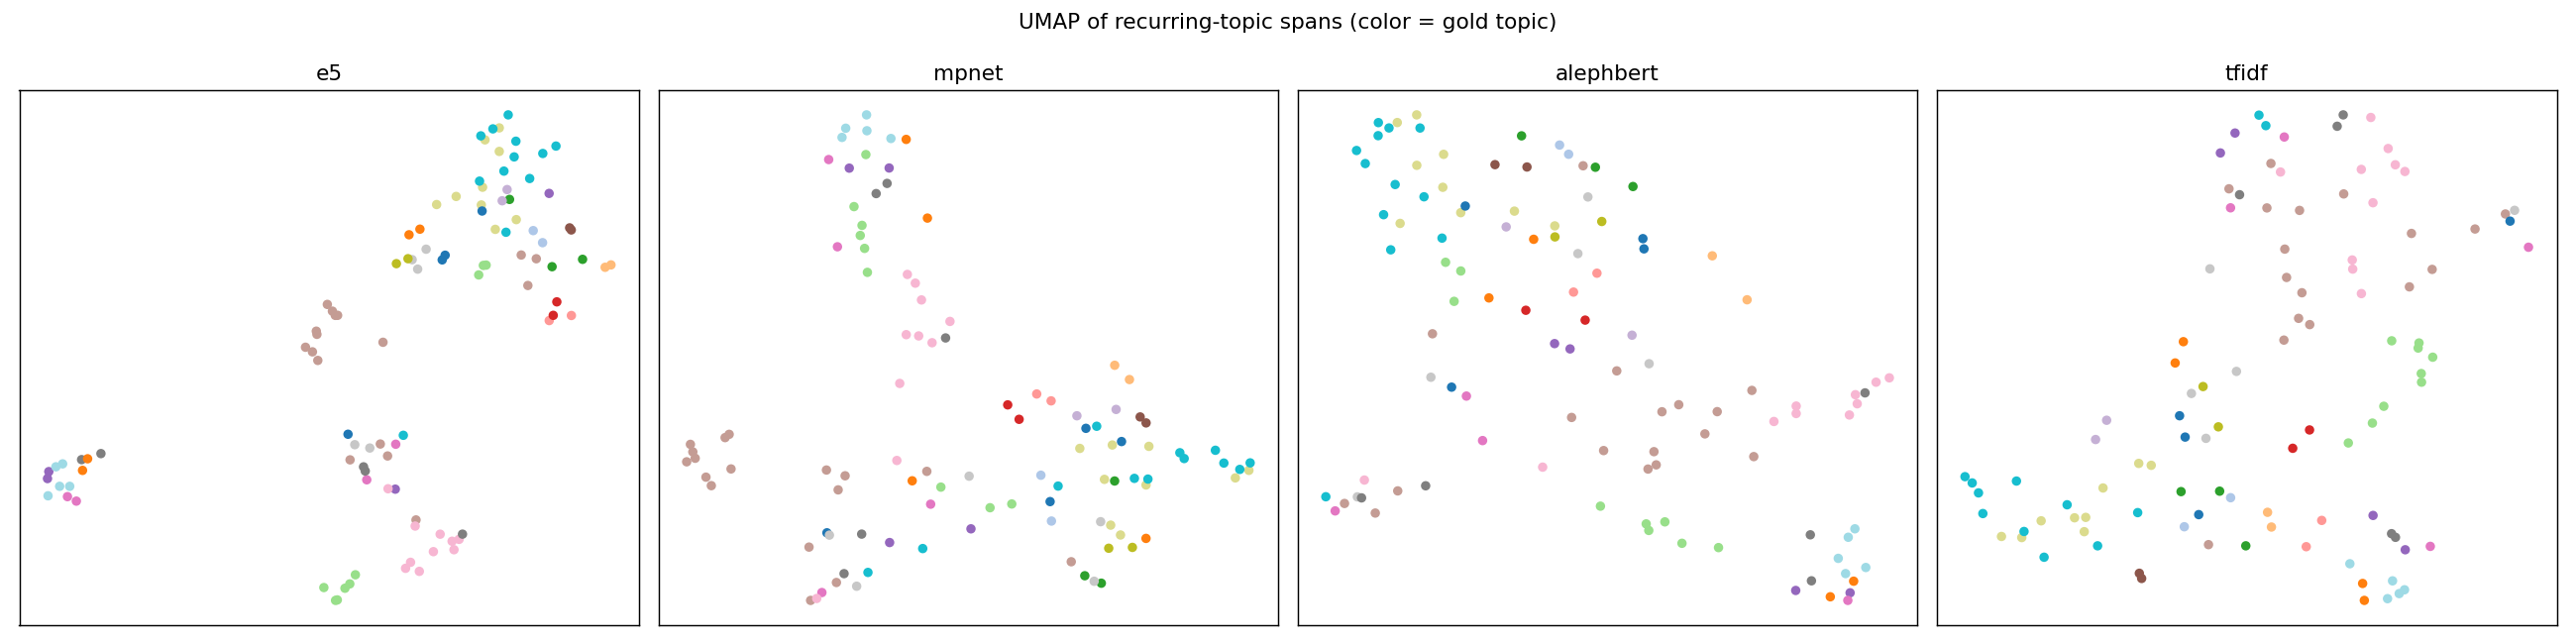
\includegraphics[width=\textwidth]{../outputs/clustering_umap.png}
\end{center}
\noindent UMAP (cosine) of the 105 recurring-topic spans, colored by gold topic. Same-color
grouping is loosest for \texttt{alephbert} (diffuse cloud) and tightest for \texttt{e5} and
\texttt{tfidf}, mirroring the quantitative ranking.

% ----------------------------------------------------------------------
\section{Takeaways}

\begin{itemize}[noitemsep]
  \item Content alone recovers topic structure only \emph{partially} (best NMI $0.80$, ARI
    $0.38$ over 28 boilerplate-heavy topics). This is a genuinely hard, ``linguistically
    adversarial'' setting --- not a deficiency of the pipeline.
  \item \textbf{Lexical $>$ semantic} here. A linking system should treat distinctive
    tokens (bill numbers, named entities) as first-class features, not rely on raw dense
    similarity.
  \item Off-the-shelf dense embeddings of single-domain Hebrew text are anisotropic and need
    correction before their cosine similarities are usable as a linking score.
\end{itemize}

% ----------------------------------------------------------------------
\section{Future Directions}

\begin{enumerate}[leftmargin=1.4em]
  \item \textbf{De-anisotropize the dense embeddings.} Mean-center and whiten (remove the top
    principal component, or apply all-but-the-top / ZCA) before cosine. This routinely widens the
    same-vs-different gap and may push e5 past TF-IDF. Cheapest high-value next experiment.
  \item \textbf{Hybrid lexical + dense score.} Combine TF-IDF (entity/number signal) with a
    corrected dense score (paraphrase robustness). A simple weighted sum or rank fusion is a
    strong candidate for the Task-2 similarity baseline.
  \item \textbf{Entity- and number-aware features.} Explicitly extract bill identifiers
    (\texttt{מ/NNNN}, \texttt{פ/NNNN}), law names, and named entities, and weight them heavily ---
    directly operationalizing the project's central hypothesis.
  \item \textbf{Character n-gram TF-IDF.} Hebrew is morphologically rich (prefixed prepositions,
    clitics); character 3--5-grams may improve lexical matching of inflected forms over word
    n-grams alone.
  \item \textbf{Discovery instead of fixed $K$.} Replace $K=28$ with HDBSCAN / a tuned cosine
    distance threshold to recover the operational setting where the number of topics is unknown
    and a ``new topic'' decision must be made online --- the actual streaming-linking task.
  \item \textbf{Segment the 20 front-loaded multi-topic protocols.} Recover their per-topic spans
    via an LLM or discourse-cue segmenter, restoring the ${\sim}30$ currently-excluded spans to the
    evaluation set.
\end{enumerate}

\vspace{1.5em}
\hrule
\vspace{0.4em}
{\small
\textbf{Artifacts (this step):}
\texttt{outputs/topic\_spans.json},
\texttt{outputs/embeddings/\{e5,mpnet,alephbert\}.npy},
\texttt{outputs/clustering\_results.json},
\texttt{outputs/clustering\_umap.png}.\\
\textbf{Code:} \texttt{code/extract\_spans.py} $\rightarrow$ \texttt{code/embed.py} $\rightarrow$ \texttt{code/cluster\_eval.py}.
}

\end{document}
